\section{Homomorphisms and subgroups}
\begin{ex}
    If $f: G \to H$ is a homomorphism of groups, then $f(e_G) = e_H$ and $f(a^{-1}) = f(a)^{-1}$ for all $a \in G$. Show by example that the first conclusion may be false if $G$, $H$ are monoids that are not groups.
\end{ex}

\begin{answer}
    For example, $(\mathbf{Z_+,+})$ and $(\mathbf{N},\times)$ are monoids. Denote $f:\mathbf{Z_+}\to \mathbf{N}$ as $f(x)=0 \forall x \in \mathbf{Z_+}$. $f$ is a homomorphism satisfies those conditions.
\end{answer}

$$ $$

\begin{ex}
    A group $G$ is abelian if and only if the map $G\to G$ given by $x\mapsto x^{-1}$ is automorphism.
\end{ex}

\begin{answer}
    If $G$ is abelian, $f(x)=x^{-1}$ is a monomorphism and epimorphism. $f(a)f(b)=a^{-1}b^{-1}=(ab)^{-1}=f(ab)$

    If $f(x)=x^{-1}$ is a isomorphism, $f(a)f(b)=a^{-1}b^{-1}=f(ab)=(ab)^{-1}=b^{-1}a^{-1} \forall a,b\in G$, so $G$ is abelian.
\end{answer}

$$ $$

\begin{ex}
    Let $Q_8$ be the group(under ordinary matrix multiplication) generated by complex matrices $A = \begin{pmatrix}
        0 & 1 \\
        -1 & 0
    \end{pmatrix}$ and $B = \begin{pmatrix}
        0 & i\\
        i & 0
    \end{pmatrix}$, where $i^{2}=-1$. Show that $Q_8$ is a nonabelian group of order 8. $Q_8$ is called the quaternion group.
\end{ex}

\begin{answer}
    The multiply operation is associative by the difinition. $A^{4}=B^{4}=\begin{pmatrix}
        1&0\\0&1
    \end{pmatrix}=I$ which is the identity element.\[A^{-1}=A^{3}=\begin{pmatrix}
        1&-1\\1&0
    \end{pmatrix}\in G\qquad B^{-1}=B^{3}=\begin{pmatrix}
        0&-i\\-i&0
    \end{pmatrix}\in G\] So $\forall A^{i}B^{j}\in G$, $(A^{i}B^{j})^{-1}\in G$. $G$ is a group. Now we examine the order of $G$ is 8.\[BA=\begin{pmatrix}
        0&i\\i&0
    \end{pmatrix}\begin{pmatrix}
        0&1\\1&0
    \end{pmatrix}=\begin{pmatrix}
        -i&0\\0&i
    \end{pmatrix}\]\[A^3B=\begin{pmatrix}
        0&-1\\1&0
    \end{pmatrix}\begin{pmatrix}
        0&i\\i&0
    \end{pmatrix}=\begin{pmatrix}
        -i&0\\0&1
    \end{pmatrix}\]So $BA=A^3B$. Take $X=A^{s_1}B^{s_2}A^{s_3}B^{s_4}\dots A^{s_{2n-1}}B^{s_{2n}}=A^{s_1}B^{s_2-1}A^3B\\A^{s_3-1}B^{s_4}\dots A^{s_{2n-1}}B^{s_{2n}}=\dots$ In finite steps , we can change it into $X=A^aB^b$. $A^{4}=B^{4}=I$, so we only consider $1\leq a,b\leq 4$. $A^{2}=B^{2}=\begin{pmatrix}
        -1&0\\0&-1
    \end{pmatrix}$, we list all: $Q_8=\{A, A^{2}, B, BA, AB, A^{2}B, AB^{2}, I\}$. The order of $Q_8$ is 8.
\end{answer}

$$ $$

\begin{ex}
    Let $H$ be the group(under ordinary matrix multiplication) of real matrices generated by $C = \begin{pmatrix}
        0 & 1\\
        -1 & 0
    \end{pmatrix}$ and $D = \begin{pmatrix}
        0 & 1\\
        1 & 0
    \end{pmatrix}$. Show that $H$ is a nonabelian group of order 8 which is not isomorphic to the quaternion group, but is isomorphic to the group $D_4^*$.
\end{ex}

\begin{answer}
    $C^{4}D^{2}=I, DC=\begin{pmatrix}
        -1&0\\0&1
    \end{pmatrix}=C^3D$.Similarly, we can prove $H$ is a nonabelian group of order 8. $H=\{C, C^{2}, C^{3}, I, D, CD, C^{2}D, C^{3}D\}$

    Assume $G\cong H$ and the isomorphism is $f$, Let $f(D)=X$, $f(D^{2})=X^{2}=f(I)=I$, so $X^{2}=I$. But $f^{-1}(I)=I\Rightarrow X\neq I\Rightarrow X=AB$ or $X=A^{2}$ or $X=B^{2}$. 
    
    If $X=A^{2}$, consider $f(C)=Y, f(C^{2}D)=Z$, we have $(Y,Z)=(B^{2},AB)$ or $(Y,Z)=(AB, B^{2})$. $f(C^{2}D)=f(C^{2})f(D)\Leftrightarrow Z=XY$. That's contradictory!

    If $X=B^{2}$, the proof is similar.

    If $X=AB$, $(Y,Z)=(A,B)$ or $(Y,Z)=(B,A)$. That's contradictory! So $f$ doesn't exist. $G$ is not isomorphic to $H$.

    Now we prove $H\cong D_4^*$. For any point $(x,y)^T$ inside the square
    \[T_x=(x,-y)^T=\begin{pmatrix}
        1&0\\0&-1
    \end{pmatrix}(x,y)^T=CD(x,y)^T\]
    \[T_y=(-x,y)^T=\begin{pmatrix}
        -1&0\\0&1
    \end{pmatrix}(x,y)^T=C^3D(x,y)^T\]
    \[T_{13}=(-y,x)^T=\begin{pmatrix}
        0&-1\\1&0
    \end{pmatrix}(x,y)^T=C^3(x,y)^T\]
    \[T_{24}=(y,-x)^T=\begin{pmatrix}
        0&1\\-1&0
    \end{pmatrix}(x,y)^T=C(x,y)^T\]
    so $D_4^*=\left\langle T_x,T_y, T_{13}, T_{24} \right\rangle=H=\left\langle C, D\right\rangle$.
\end{answer}

$$ $$

\begin{ex}
    Let $S$ be a nonempty subset of a group $G$ and define a relation on $G$ by $a \thicksim b$ if and only if $ab^{-1}\in S$. Show that $\thicksim$ is an equivalence relation if and only if $S$ is a subgroup of $G$.
\end{ex}

\begin{answer}
    If $\thicksim$ is a equivalence relation
    \begin{enumerate}
        \item $a\thicksim b\Rightarrow b\thicksim a$;
        \item $a\thicksim a$;
        \item $a\thicksim b, b\thicksim c\Rightarrow a\thicksim c$.
    \end{enumerate}
    $2\Leftrightarrow aa^{-1}=e\in S$. $1\Rightarrow a\thicksim e\Rightarrow e \thicksim a\forall a\in S$, so $ ae^{-1}=a\in S, ea^{-1}=a^{-1}\in S$. If $a,b\in S, b^{-1} \in S$, so $ae^{-1}\in S, e(b^{-1})^{-1}\in S$. By 3, $a\thicksim e, e\thicksim b^{-1}\Rightarrow a\thicksim b^{-1}\Rightarrow ab\in S$. $S$ is a subgroup of $G$.

    If $S$ is a subgroup of $G$
    \begin{enumerate}
        \item $aa^{-1}\in S\Rightarrow a\thicksim a$;
        \item $ab^{-1}\in S\Rightarrow (ab^{-1})^{-1}=ba^{-1}\in S\Rightarrow (a\thicksim b\Rightarrow b\thicksim a)$;
        \item $ab^{-1}\in S,bc^{-1}\in S\Rightarrow (ab^{-1})(bc^{-1})=ac^{-1}\in S$, which means $a\thicksim b,b \thicksim c\Rightarrow a\thicksim c$
    \end{enumerate}
    In conclusion, $\thicksim$ is a equivalence relation.
\end{answer}

$$ $$

\begin{ex}
    A nonempty finte subset of a group is s subgroup if and only if it is closed under the product in $G$.
\end{ex}

\begin{answer}
    $\Rightarrow$: Trivial.

    $\Leftarrow$: $S$ is apparently associative. $\forall a,b\in S, ab\in S$. $S$ is a finite set, so there exists $m>n\in \mathbf{N}$ s.t. $a^{m}=a^{n}$. %TODO
\end{answer}

$$ $$

\begin{ex}
    If $n$ is a fixed integer, then $\{kn | n\in \mathbf{Z}\}\subset\mathbf{Z}$ is an additive subgroup of $\mathbf{Z}$, which is isomorphic to $\mathbf{Z}$. 
\end{ex}

\begin{answer}
    Denote $Z^{n}=\{kn|k\in\mathbf{Z}\}$. We can easily check that $Z^n$ is a subgroup of $\mathbf{Z}$. Now we build a isomorphism between $Z^{n}$ and $\mathbf{Z}$. Take $f:Z^{n}\to\mathbf{Z}$ as $f(kn)=k$, $f^{-1}(n)=kn$. $f$ is a bijection so $Z^{n}$ and $\mathbf{Z}$ are isomorphism.
\end{answer}

$$ $$

\begin{ex}
    The set $\{\sigma\in S_n | \sigma(n) = n\}$ is a subgroup of $S_n$ which is isomorphic to $S_{n-1}$.
\end{ex}

\begin{answer}
    Denote $S_n^{(n)}=\{\sigma\in S_n|\sigma(n)=n\}$. $\forall \sigma_1,\sigma_{2}\in S_n^{(n)}, \sigma_{1}\sigma_{2}(n)=\sigma_1(\sigma_{2}(n))=\sigma_{1}(n)=n$, so $\sigma_{1}\sigma_{2}\in S_n^{(n)}$. By the above exercise, $S_n^{(n)}$ is a subgroup of $S_n$. Now we build an isomorphism between $S_n^{(n)}$ and $S_{n-1}$.
    Take $f: S_{n-1}\to S_n^{(n)}$ as $f(\sigma) =\sigma'$, where $\sigma'(x)=\left\{\begin{aligned}
        &n, &x=n\\ &\sigma(n), &x\neq n
    \end{aligned}\right.$. $\sigma'\in S_n^{(n)}$ and $f$ is a bijection, so $S_{n-1}\cong S_n^{(n)}$.
\end{answer}

$$ $$

\begin{ex}
    Let $f: G\to H$ be a homomorphism of groups, $A$ a subgroup of $G$, and $B$ a subgroup of $H$.
    \begin{enumerate}
        \item $\mathrm{Ker} f$ and $f^{-1}(B)$ are subgroups of $G$.
        \item $f(A)$ is a subgroup of $H$.
    \end{enumerate}
\end{ex}

\begin{answer}
    \begin{enumerate}
        \item $f$ is a homomorphism, so $f(e)=e', e\in \mathrm{Ker} f$. $\forall a \in 
    \mathrm{Ker} f$, $f(aa^{-1})=f(a)f(a^{-1})=e'$, so $f(a^{-1})=f(a)^{-1}=e'^{-1}=e'$. $\forall a,b \in \mathrm{Ker} f, f(ab^{-1})=f(a)f(b^{-1})=f(a)f(b)^{-1}=e'\Rightarrow ab^{-1}\in \mathrm{Ker} f$, which means $\mathrm{Ker} f$ is a subgroup of $G$. The proof of $f^{-1}(B)$ is a subgroup of $G$ is similar.
        \item $f$ is a homomorphism, $f(e)=e'$. $\forall a,b\in A, ab^{-1}\in A$, so $f(ab^{-1})=f(a)f(b^{-1})=f(a)f(b)^{-1}\in f(A)$, $f(A)$ is a subgroup of $H$.
    \end{enumerate}
\end{answer}

$$ $$

\begin{ex}
    List all subgroups of $Z_2\oplus Z_2$. Is $Z_2\oplus Z_2$ isomorphic to $Z_4$?
\end{ex}

\begin{answer}
    $Z_2\oplus Z_2$: $\{\{(1,1),(1,0),(0,1),(0,0)\},\{(1,1),(0,0)\},\{(0,0)\},\\\{(1,0),(0,0)\},\{(0,1),(0,0)\},\{(0,1),(1,0),(0,0)\}\}$.

    $Z_4$: $\{\{\bar{0}, \bar{1}, \bar{2}, \bar{3}\}, \{\bar{0}, \bar{2}\}, \{\bar{0}\}\}$.

    $Z_4$ and $Z_2\oplus Z_2$ are not isomorphic because they have different subgroups.
\end{answer}

$$ $$

\begin{ex}
    If $G$ is a subgroup, then $C = \{a\in G| ax = xa \text{ for all } x\in G\}$ is a abelian subgroup of $G$. $C$ is called the center of $G$.
\end{ex}

\begin{answer}
    Take $a,b\in C, ab=ba$, $C$ is communicative. $\forall  a,b\in C, x\in G$, $b^{-1}\in G$, so $ab^{-1}=b^{-1}a$.\[ax=axbb^{-1}=abxb^{-1}=baxb^{-1}=bxab^{=1}=abb^{-1}x=bab^{-1}x\]so $b^{-1}ax=ab^{-1}x=xab^{-1}$, $ab^{-1}\in C$, $C$ is a subgroup of $G$.
\end{answer}

$$ $$

\begin{ex}
    The group $D_4^*$ is not cyclic, but can be generated by two elements. The same is true of $S_n$(nontrivial). What is the minimal number of generators of the additive group $\mathbf{Z}\oplus\mathbf{Z}$?
\end{ex}

\begin{answer}
    $\mathbf{Z}\oplus\mathbf{Z}=\{(a,b)|a\in \mathbf{Z}, b\in\mathbf{Z}\}=\left\langle(0,0), (1,0), (0,1)\right\rangle$. We can easily check the spanning set is the minimal.
\end{answer}

$$ $$

\begin{ex}
    If $G = \left\langle a \right\rangle $ is a cyclic group and $H$ is any group, then every homomorphism $f:G\to H$ is completely determined by the element $f(a)\in H$.
\end{ex}

\begin{answer}
    $\forall x\in G$, there exist $m\in \mathbf{N}$ s.t. $x=a^{m}$, so $f(x)=f(a^{m})=f(a)^{m} \Rightarrow \mathrm{Im} f=\left\langle f(a)\right\rangle$. $f:a^{m}\mapsto f(a)^{m} \forall m\in\mathbf{N}$. $f$ is completely determined by $f(a)\in H$.
\end{answer}

$$ $$

\begin{ex}
    The following cyclic subgroups are all isomorphic: the multiplication group $\left\langle i \right\rangle$ in $\mathbf{C}$, the additive group $\mathbf{Z_4}$ and the subgroup $\left\langle \begin{pmatrix}
        1 & 2 & 3 & 4\\
        2 & 3 & 4 & 1
    \end{pmatrix}\right\rangle$ of $S_4$.
\end{ex}

\begin{answer}
    $\left\langle i\right\rangle=\{i,-1,-i,1\}$, $Z_4=\{\bar{0},\bar{1},\bar{2},\bar{3}\}$,\\ $\left\langle(1234)\right\rangle=\{(1234),(13)(24),(1432),(1)\}$.
    Denote $f: \left\langle i\right\rangle\to Z_4$ as $f(i)=\bar{i}$, $g: Z_4\to \left\langle(1234)\right\rangle$ as $g(i)=(1234)$. From the exercise above we know $f$ and $g$ aer homomorphisms, and they are bijections, so $\left\langle i\right\rangle\cong Z_4\cong\left\langle(1234)\right\rangle$.
\end{answer}

$$ $$

\begin{ex}
    Let $G$ be a group and $\mathrm{Aut} G$ is the set of all automorphisms of $G$.
    \begin{enumerate}
        \item $\mathrm{Aut} G$ is a group with composition of functions as binary operation.
        \item $\mathrm{Aut} \mathbf{Z}\cong Z_2$ and $\mathrm{Aut} Z_6 \cong Z_2$; $\mathrm{Aut} Z_8\cong Z_2\oplus Z_2$; $\mathrm{Aut} Z_p\cong Z_{p-1}$ ($p$ prime).
        \item What is $\mathrm{Aut Z_n}$ for arbitrary $n\in \mathbf{N^*}$?
    \end{enumerate}
\end{ex}

\begin{answer}
    We only prove the third question.

    For $\bar{a}\in Z_{n}$, the order of $\bar{a}$ is $\left| \bar{a} \right|=\frac{n}{(n,a)}$. When $(n,a)=1$, $\bar{a}$ is a generator of $Z_{n}$. Denote Euler function as $\varphi(x)$ and $Z_{n}^{*}=\{\bar{a}\in Z_{n}|(a,n)=1\}$, then $\left| Z_{n}^{*} \right| =\varphi(n)$. For $\sigma \in \mathrm{Aut}Z_{n}$, $\sigma$ is completely determined by $\sigma(\bar{1})=\bar{a}$, and we denote $\sigma$ as $\sigma_{a}$. For $\sigma_{a},\sigma_{b}\in \mathrm{Aut}Z_{n}$, $\sigma_{a}(\sigma_{b}(\bar{1}))=\sigma_{a}(\bar{b})=\bar{ab}=\sigma_{ab}(\bar{1})$. We have proved $\mathrm{Aut}Z_{n}\cong Z_{n}^{*}$.

    Now we give out a lemma to show the structure of $Z_{n}^{*}$.
    \begin{lemma}
        If $n=st, (s,t)=1$, then $Z_{n}^{*}\cong Z_{s}^{*}\oplus Z_{t}^{*}$.
    \end{lemma}
    The proof of this lemma is quite simple. Consider the mappping $f^{*}: Z_{n}^{*}\to Z_{s}^{*}\oplus Z_{t}^{*}$ which is defined by $(x \mod n)\mapsto (x\mod s, x\mod t)$. Since for any $a,b\in Z_{n}^{*}$, $f^{*}(a)f^*(b)=(a\mod s,a\mod t)(b\mod s,b\mod t)=(ab\mod s,ab\mod t)=f^{*}(ab)$, $f^{*}$ is a well defined homomorphism. For $x\in \mathrm{Ker}f^{*}$, $x\equiv 1\mod s$, $x\equiv 1\mod t$, so $x\equiv 1\mod \left[s,t\right]$, $x\equiv 1\mod n$, $f^{*}$ is a monomorphism. Since $\left| f^{*}(Z_{n}^{*}) \right|=\left| Z_{n} \right| =\varphi(n)=\varphi(s)\varphi(t)=\left| Z_{s}^{*}\oplus Z_{t}^{*} \right|$, $f^{*}$ is a epimorphism. $Z_{n}^{*}\cong Z_{s}^{*}\oplus Z_{t}^{*}$ 

    For $n=p_{1}^{k_{1}}p_{2}^{k_{2}}\cdots p_{m}^{k_{m}}$, $Z_{n}^{*}\cong Z_{p_{1}^{k_{1}}}^{*}\oplus Z_{p_{2}^{k_{2}}}^{*}\oplus\cdots\oplus Z_{p_{m}^{k_{m}}}^{*}$. Now we consider the structure of $Z_{p^{k}}^{*}$. 

    For $p=2$, $Z_{2}^{*}\cong Z_{1}$, $Z_{4}^{*}\cong Z_{2}$, $Z_{2^{k}}^{*}\cong Z_{2}\oplus Z_{2^{k-2}}$.

    For other odd prime $p$, $Z_{p^{k}}^{*}\cong Z_{(p-1)p^{k-1}}$.

    In order to prove the result, we need the Lagrange theorem in number theory.

    \begin{lemma}[Lagrange]
        $f(x)\in Z\left[n\right]$, $f(x)\equiv k$ has at most $n$ solutions when $\mod p$, where $p$ is an odd prime.
    \end{lemma}

    We use induction to prove the lemma.

    \begin{enumerate}
        \item $n=1$, the proof the trivial.
        \item Assume for $n\leq m-1$ the lemma is correct, and for $n= m$, $f(x)\equiv k$ has $m+1$ solutions. $f(x)-f(x_{m+1})=(x-x_{m+1})g(x)\equiv 0\mod p$. Take $x=x_{i}, i=1,2,\dots ,m$, $(x_{i}-x_{m+1})g(x_{i})\equiv 0\mod p$, $x_{i}\neq x_{m+1}$, so $g(x_{i})\equiv 0\mod p$, That's contradictory to the induction assumptions! 
    \end{enumerate}
    The lemma is proved.

    Come back to the original question. Firstly, we consider $k=1$ and $p$ is an odd prime. For any factor $d$ of $p-1$, denote $S(d)=\{\bar{a}\in Z_{p}^{*}|\mathrm{ord}_p(a)=d\}$. $S(d)$ forms a partition of $Z_{p}^{*}$. If $S(d)\neq \emptyset$, there exists $\bar{a}\in S(d)$ and $a^{d}\equiv 1\mod p$. By Largrange theorem, $a^{d}\equiv 1\mod p$ has at most $d$ solutions. Notice that $\{1,a,a^{2},\dots, a^{d-1}\}$ are the solutions of the equation, $a^{i}\equiv \!\!\!\!\!\!/a^{j}\mod p$, whence $S(d)\subset\left\langle\bar{a}\right\rangle$. For $k=1,2,\dots,d-1$, $\mathrm{ord}_p(\bar{a^{k}})=\left| a^{k} \right| =\frac{d}{(d,k)}=d\Leftrightarrow(d,k)=1$. Thus $\left| S(d) \right| =\varphi(d)$.

    From $Z_{p}^{*}=\bigcup\limits_{d|p-1}S(d)$, we get \[p-1=\left| Z_{p}^{*} \right| =\sum\limits_{d|p-1}\left| S(d) \right| \leq \sum_{d|p-1}\varphi(d)=p-1\] If $d|p-1$, $\left| S(d) \right| =\varphi(d)$. Particularly, when $d=p-1$, $\left| S(p-1) \right| =\varphi(p-1)\neq 0$, $Z_{p}^{*}$ has a element of order $p-1$, $Z_{p}^{*}$ is a cyclic group.

    Secondly, we consider $k\geq 2$. Take $a\in\mathbf{Z}$ and $\bar{a}$ is the class of $x\equiv a\mod p^{k}$. For $s\geq t$, we have a group homomorphism $f_{s,t}:Z_{p^{s}}^{*}\to Z_{p^{t}}^{*}$ which is defined by $(a \mod p^{s})\mapsto (a\mod p^{t})$. Since $a\equiv b\mod p^{s}\Rightarrow a\equiv b\mod p^{t}$, $f$ is well defined. $\mathrm{Ker}f_{s,t}=\{up^{t}+1\mod p^{s}|u=0,1,\dots,p^{s-t}-1\}$. If $2t\geq s$, since $(up^{t}+1)(vp^{t}+1)\equiv uvp^{2t}+(u+v)p^{t}+1\equiv (u+v)p^{t}+1\mod p^{s}$, $\mathrm{Ker}f_{s,t}\cong Z_{p^{s-t}}$ is a cyclic group. There exists a isomorphism $g_{s,t}:Z_{p^{s}}^{*}/\mathrm{Ker}f_{s,t}\to Z_{p^{t}}^{*}$. \[\{\bar{1}_{p^{k}}\}=\mathrm{Ker}f_{k,k}<\mathrm{Ker}f_{k,k-1}<\cdots<\mathrm{Ker}f_{k,1}<Z_{p^{k}}^{*}\] 
    \begin{lemma}
        Suppose $i\geq 2$, $\bar{a}_{p^{k}}\in\mathrm{Ker}f_{k,i}$, but $\bar{a}_{p^{k}}\notin \mathrm{Ker}f_{k,i+1}$, then $\bar{a}_{p^{k}}^{p}\in \mathrm{Ker}f_{k,i+1}$ and $\bar{a}_{p^{k}}^{p}\notin \mathrm{Ker}f_{k,i+2}$.
    \end{lemma}
    This lemma can be proved by LTE. Here we use the language in group theory to prove it. $f_{k,i+2}(\bar{a}_{p^{k}})=\bar{a}_{p^{i+2}}$, $\bar{a}_{p^{i+2}}\in f_{k,i+2}(\mathrm{Ker}f_{k,i})=\mathrm{Ker}f_{i+2,i}$. $\mathrm{Ker}f_{i+2,i}\cong Z_{p^{2}}$ since $2i\geq i+2$. $\bar{a}_{p^{i+2}}\notin f_{k,i+2}(\mathrm{Ker}f_{k,i+1})=\mathrm{Ker}f_{i+2,i+1}\cong Z_{p}$. $\mathrm{Ker}f_{i+2,i+1}$ contains all the elements whose order is $p$ in $\mathrm{Ker}f_{i+2,i}$, so $\left| \bar{a}_{p^{i+2}} \right| =p^{2}$. $\bar{a}_{p^{i+2}}^{p}\in \mathrm{Ker}f_{i+2,i+1}$, $\bar{a}_{p^{i+2}}^{p}\notin \mathrm{Ker}f_{i+2,i+2}$, $\bar{a}_{p^{k}}^{p}\in g_{k,i+2}^{-1}(\bar{a}_{p^{i+2}}^{p})\subset g_{k,i+2}^{-1}(\mathrm{Ker}f_{i+2,i+1})=\mathrm{Ker}f_{k,i+1}$, $\bar{a}_{p^{k}}^{p}\notin g_{k,i+2}^{-1}(\mathrm{Ker}f_{i+2,i+2})=\mathrm{Ker}f_{k,i+2}$.

    For $i=1$, if $p$ is an odd prime, $\mathrm{Ker}f_{3,1}=\left\langle\bar{p+1}_{p^{3}}\right\rangle\cong Z_{p^{2}}$, if $p=2$, $\mathrm{Ker}f_{3,1}=\{\bar{1}_{8},\bar{3}_{8},\bar{5}_{8},\bar{7}_{8}\}\cong Z_{2}\oplus Z_{2}$. Thus, for $\bar{a}_{p^{k}}\in\mathrm{Ker}f_{k,2}, \bar{a}_{p^{k}}\notin \mathrm{Ker}f_{k,3}$, using the lemma above for several times, we get $\bar{a}_{p^{k}}^{p^{k-2}}\in\mathrm{Ker}f_{k,2},\bar{a}_{p^{k}}^{p^{k-3}}\notin\mathrm{Ker}f_{k,k}$, $\left| \bar{a}_{p^{k}} \right|=p^{k-2} $, $\mathrm{Ker}f_{k,2}\cong Z_{p^{k-2}}$.

    If $p$ is an odd prime, we can further obtain $\mathrm{Ker}f_{k,1}\cong Z_{p^{k-1}}$.

    Suppose $x$ is a generator of $Z_{p}^{*}$, assume $a\in g_{k,1}^{-1}(x)$, $g_{k,1}^{-1}(x)=a\mathrm{Ker}f_{k,1}$, and $a^{p-1}\in g_{k,1}^{-1}(x^{p-1})=g_{k,1}^{-1}(\bar{1}_{p})=\mathrm{Ker}f_{k,1}$. If $a^{p-1}\notin \mathrm{Ker}f_{k,2}$, then $\left| a^{p-1} \right| =p^{k-1}$. If $a^{p-1}\in \mathrm{Ker}f_{k,2}$, $\forall h\in \mathrm{Ker}f_{k,1},h \notin\mathrm{Ker}f_{k,2}$. Since $(ah)^{p-1}=(a^{p-1}h^{p})h^{-1}$, $(ah)^{p-1}\in \mathrm{Ker}f_{k,1}, (ah)^{p-1}\notin \mathrm{Ker}f_{k,2}$, whence $\left| (ah)^{p-1} \right|=p^{k-1} $, $Z_{p^{k}}^{*}\cong Z_{(p-1)p^{k-1}}$.

    If $p=2$, $Z_{2^{k}}^{*}=\mathrm{Ker}f_{k,1}\cong Z_{2^{k-2}}\oplus Z_{2}$.

    For $\mathrm{Aut}\mathbf{Z}$, assume there exist $f\neq 1_{G}, -1_{G}$, $f\in \mathbf{Aut}\mathbf{Z}$. WLOG, $f(1)=x\neq \pm 1, f(-1)=y$. $f(1)+f(-1)=f(0)=x+y=0$. Assume $af(1)+bf(-1)=f(a-b)=1=(a-b)x$, since $x\neq \pm 1$, there is a contradiction. $\mathrm{Aut}\mathbf{Z}\cong Z_{2}$.
\end{answer}

$$ $$

\begin{ex}
    For each prime $p$ the additive subgroup $Z(p^\infty)$ of $\mathbf{Q}/\mathbf{Z}$ is generated by the set $\{\bar{1/p^n}|n\in \mathbf{N^*}\}$.
\end{ex}

\begin{answer}
    We prove that $\left\langle\bigcup\limits_{n=1}^{\infty}\frac{1}{p^{n}}\right\rangle\cong Z(p^{\infty})$. $\forall x\in Z(p^{\infty}), x=\bar{\frac{a}{b}}=\bar{\frac{a}{p^{k}}}$. Expand $a$ as $a=\sum\limits_{i=0}^{k-1}p^{i}a_{i}$, where $a_{i}=1,2,\dots n-1$. $x=\bar{\frac{a}{b}}=\sum\limits_{i=0}^{k-1}\bar{\frac{a_{i}}{p^{k-i}}}=\sum\limits_{i=1}^{k}\bar{\frac{a_{k-i}}{p^{i}}}$. Denote $f: \left\langle\bigcup\limits_{n=1}^{\infty}\frac{1}{p^{n}}\right\rangle\to Z(p^{\infty})$ as $f(\sum\limits_{i=1}^{n}\frac{a_{i}}{p^{i}})=\bar{\sum\limits_{i=1}^{n}\frac{a_{i}}{p^{i}}}$. $f$ is an isomorphism because every $x\in Z(p^{\infty})$ can be written in such form.
\end{answer}

$$ $$

\begin{ex}
    Let $G$ be an abelian group and let $H, K$ be subgroups of $G$. Show that the join $H\vee K$ is the set $\{ab|a\in H, b\in K\}$. Extend this result to any finite number of subgroups of $G$.
\end{ex}

\begin{answer}
    $H\vee K=\left\langle H\cup K\right\rangle, I=\{ab| a\in H,b\in K\}$. $G$ is abelian so $I$ is a subgroup of $G$. $H<I, K<I, (H\cup K)\subset I$. $\left\langle H\cup K\right\rangle\subset I\Rightarrow \left\langle H\cup K\right\rangle$.

    For any $ab\in I$, $a\in H$, $b\in K$, we prove that $ab$ is contained in any subgroup which contains $H\cup K$.

    Assume $(H\cup K)\subset J$, so $a\in J, b\in J\Rightarrow ab\in J$, which means $I\subset H\vee K$. $\left\langle H\cup K\right\rangle = I$.

    $G$ is abelian group, $H_1, H_2,\dots H_n$ are $n$ subgroups. $\left\langle\bigcup\limits_{i=1}^{n}H_i\right\rangle=\{\prod\limits_{i=1}^{n}h_{i}|h_{i}\in H_{i},i=1,2,\dots n\}$. This proposition can be proved by induction.
\end{answer}

$$ $$

\begin{ex}
    \begin{enumerate}
        \item Let $G$ be a group and $\{H_i| i\in I\}$ a family of subgroups. State and prove a condition that will imply that $\bigcup\limits_{i\in I}H_i$ is a subgroup, that is $\bigcup\limits_{i\in I}H_i = \left\langle\bigcup\limits_{i\in I}H_i\right\rangle$.
        \item Given an example of a group $G$ and a family of subgroups $\{H_i|i \in I\}$ such that $\bigcup\limits_{i\in I}H_i \neq \left\langle\bigcup\limits_{i\in I}H_i\right\rangle$.
    \end{enumerate}
\end{ex}

\begin{answer}
    I didn't find a sufficient and necessary condition for this question, just choose one as you like:)
\end{answer}

$$ $$

\begin{ex}
    \begin{enumerate}
        \item The set of all subgroups of a group $G$, partially ordered by set theoretic inclusion, forms a complete lattice in which the g.l.b of $\{H_i|i\in I\}$ is $\bigcap\limits_{i\in I}H_i$ and the l.u.b is $\left\langle\bigcap\limits_{i\in I}H_i\right\rangle$.
        \item Exhibit the lattice of subgroups of the groups $S_3, D_4^*, Z_6, Z_{27}$ and $Z_{36}$.
    \end{enumerate}
\end{ex}

\begin{answer}
    \begin{enumerate}
        \item The subset relation $<$ forms a partially ordered relation. By the difinition of $\left\langle\bigcup\limits_{i\in I}H_i\right\rangle$, $\left\langle\bigcup\limits_{i\in I}H_i\right\rangle$ is the smallest set contains $\bigcup\limits_{i\in I}H_i$, so it's lup. For glb, we know that $\bigcap\limits_{i\in I}H_i\subset H_i \,\,\forall i\in I$, and $\forall H\supset \bigcap\limits_{i\in I}H_i$, there exists $x\in H, x\notin H_j \,\,j\in I$, so $\bigcap\limits_{i\in I}$ is glb.
        \item  $S_3=\{(1), (12), (13), (23), (123), (132)\}$.
        \begin{figure}[H]\centering
            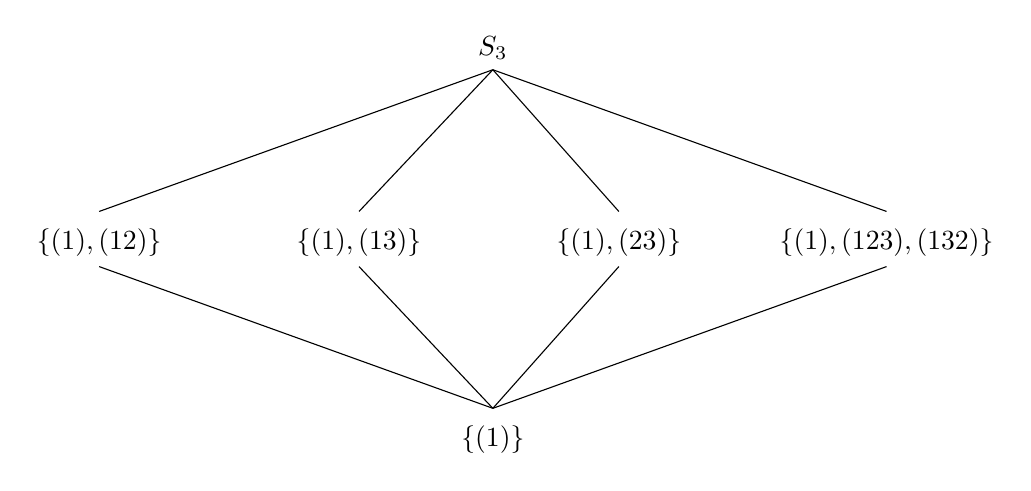
\begin{tikzpicture}
                \node [above] at (5,5) {$S_{3}$};
                \node [above] at (0, 2.5) {$\{(1),(12)\}$};
                \node [above] at (3.3, 2.5) {$\{(1),(13)\}$};
                \node [above] at (6.6, 2.5) {$\{(1),(23)\}$};
                \node [above] at (10, 2.5) {$\{(1),(123),(132)\}$};
                \node [above] at (5,0) {$\{(1)\}$};
                \draw [-] (5,5) -- (0, 3.2);
                \draw [-] (5,5) -- (3.3, 3.2);
                \draw [-] (5,5) -- (6.6, 3.2);
                \draw [-] (5,5) -- (10, 3.2);
                \draw [-] (5,0.7) -- (0, 2.5);
                \draw [-] (5,0.7) -- (3.3, 2.5);
                \draw [-] (5,0.7) -- (6.6, 2.5);
                \draw [-] (5,0.7) -- (10, 2.5);
            \end{tikzpicture}
        \end{figure}

        $D_4^*=\{R, R^{2}, R^{3}, I, T_{x}, T_{y}, T_{13}, T_{24}\}$.

        \begin{figure}[H]\centering
            \begin{tikzpicture}
                \node [above] at (3.5,6) {$D_{4}^{*}$};
                \node [above] at (3.5,4) {$\{R,R^{2},R^{3},I\}$};
                \node [above] at (0,4) {$\{I, R^{2}, T_{x}, T_{y}\}$};
                \node [above] at (7,4) {$\{I, R^{2}, T_{13}, T_{24}\}$};
                \node [above] at (3.5,2) {$\{I, R^{2}\}$};
                \node [above] at (3.5,0) {$\{I\}$};
                \draw [-] (3.5,6) to (0,4.7);
                \draw [-] (3.5,6) to (3.5,4.7);
                \draw [-] (3.5,6) to (7,4.7);
                \draw [-] (3.5,2.7) to (0,4);
                \draw [-] (3.5,2.7) to (3.5,4);
                \draw [-] (3.5,2.7) to (7,4);
                \draw [-] (3.5,2) to (3.5,0.7);
            \end{tikzpicture}
        \end{figure}

        $Z_6=\{\bar{0},\bar{1},\bar{2},\bar{3},\bar{4},\bar{5}\}$.

        \begin{figure}[H]\centering
            \begin{tikzpicture}
                \node [above] at (2.5,5) {$Z_{6}$};
                \node [above] at (0,2.5) {$\{\bar{0},\bar{3}\}$};
                \node [above] at (5,2.5) {$\{\bar{0},\bar{2},\bar{4}\}$};
                \node [above] at (2.5,0) {$\{\bar{0}\}$};
                \draw [-] (2.5,5) -- (0,3.2);
                \draw [-] (2.5,5) -- (5,3.2);
                \draw [-] (2.5,0.8) -- (0,2.5);
                \draw [-] (2.5,0.8) -- (5,2.5);
            \end{tikzpicture}
        \end{figure}
    \end{enumerate}
\end{answer}